\lab{Algorithms}{Profiler and Structs}{Profiler and Structs}

\objective{Learn how to use Structs in MATLAB, and how to use the profiler to optimize code.}

Often physical models have many parameters. MATLAB offers a simple way to handle groups of parameters, known as a structure. Try the following:

\begin{lstlisting}[style=matlab]
P.a = 10;
P.b = 3;
\end{lstlisting}

Now instead of passing the parameters a and b, you can simply pass the structure P and then access the parameters. This makes our functions much easier to use, and it makes paramters much easier to manipulate.

For example, consider the following dynamical system (known as the Lotka-Volterra equation):

\begin{equation}
    \begin{split}
        R'(t) &=aR(t)-bR(t)F(t)\\
        F'(t) &=cR(t)F(t)-dF(t)
    \end{split}\notag
\end{equation}

This system represents predator-prey interaction. $R$ is the number of prey, and $F$ is the number of predators. Suppose that we want to run this model with varying parameters. We can do this very easily with structures:

\begin{lstlisting}[style=matlab]
P.a = 10;
P.b = 3;
P.c = 2;
P.d = 1;
f = @(t,x) [P.a*x(1)-P.b*x(1)*x(2); P.c*x(1)*x(2) - P.d*x(2)];
[t y] = ode45(f,[0 10],[7;7]);
\end{lstlisting}

\begin{problem}
Write a function Lotka(t,P) that plots the solution of the Lotka-Volterra equation on the interval $[0,t]$ using parameters stored in structure P. 
\end{problem}

Next we will introduce a powerful tool in code optimization: the Profiler. At the command line in MATLAB type ``profile viewer''. You should see a window that looks like this:

\begin{center}
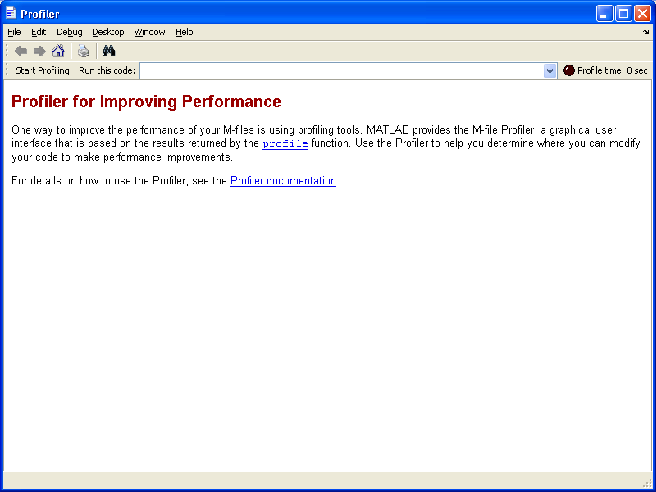
\includegraphics[scale = .7]{./Figures/blankProfile}
\end{center}

This is the profiler. Now run Lotka(25,P), with some P that you set previously. You should get output that looks like this:

\begin{center}
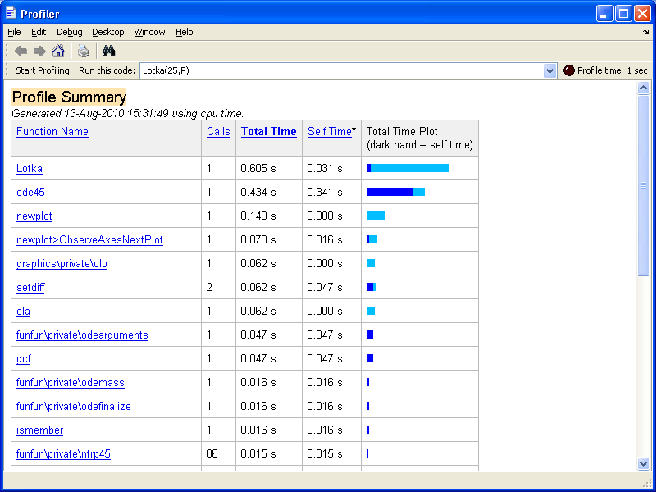
\includegraphics[scale = .7]{./Figures/LotkaProfile}
\end{center}

Explore this window. Try clicking on some of the links. You can view how long MATLAB spent calling different functions trying to solve this differential equation.

This information can be incredibly valuable in speeding up functions. You can clearly see what functions are being called, and where speed-up needs to occur.

\begin{problem}
Write the following function:
\begin{lstlisting}[style=matlab]
function I = interpquad(x,y)
%%This function interpolates sorted data points and then integrates the function found by interpolation
method = 'pchip';
I = quad(@interpolant,x(1),x(end));

    function f = interpolant(t)
            f = interp1(x,y,t,method); 
\end{lstlisting}

Run the profiler on this function, using the following code to generate your random data:

\begin{lstlisting}[style=matlab]
x = 1:.2:10;
y = log(x) + rand(size(x))-.5
\end{lstlisting}

What do you notice? How many times is \li{interp1} called? This is a problem, since \li{interp1} has to calculate the interpolating function every time it is called. Look up the 'pp' option in the help documentation of \li{interp1}. Apply this option so that \li{interp1} is only called once. How much does performance improve?
\end{problem}


